% Created by tikzDevice version 0.6.2-92-0ad2792 on 2012-09-26 20:23:29
% !TEX encoding = UTF-8 Unicode
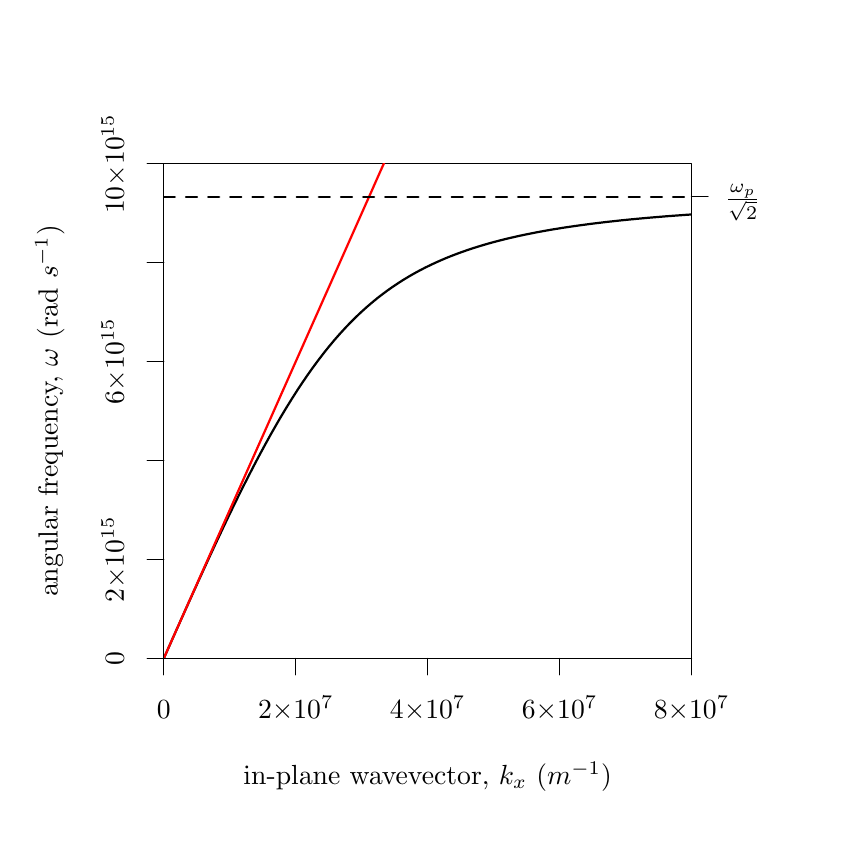
\begin{tikzpicture}[x=1pt,y=1pt]
\definecolor[named]{fillColor}{rgb}{1.00,1.00,1.00}
\path[use as bounding box,fill=fillColor,fill opacity=0.00] (0,0) rectangle (289.08,289.08);
\begin{scope}
\path[clip] (  0.00,  0.00) rectangle (289.08,289.08);
\definecolor[named]{drawColor}{rgb}{0.00,0.00,0.00}

\path[draw=drawColor,line width= 0.4pt,line join=round,line cap=round] ( 49.20, 61.20) --
	(239.88, 61.20) --
	(239.88,239.88) --
	( 49.20,239.88) --
	( 49.20, 61.20);
\end{scope}
\begin{scope}
\path[clip] (  0.00,  0.00) rectangle (289.08,289.08);
\definecolor[named]{drawColor}{rgb}{0.00,0.00,0.00}

\node[text=drawColor,anchor=base,inner sep=0pt, outer sep=0pt, scale=  1.00] at (144.54, 15.60) {in-plane wavevector, $k_x$ ($m^{-1}$)};

\node[text=drawColor,rotate= 90.00,anchor=base,inner sep=0pt, outer sep=0pt, scale=  1.00] at ( 10.80,150.54) {angular frequency, $\omega$ (rad $s^{-1}$)};
\end{scope}
\begin{scope}
\path[clip] ( 49.20, 61.20) rectangle (239.88,239.88);
\definecolor[named]{drawColor}{rgb}{0.00,0.00,0.00}

\path[draw=drawColor,line width= 0.8pt,line join=round,line cap=round] ( 49.20, 61.20) --
	( 51.13, 65.53) --
	( 53.05, 69.86) --
	( 54.98, 74.18) --
	( 56.90, 78.48) --
	( 58.83, 82.77) --
	( 60.76, 87.03) --
	( 62.68, 91.27) --
	( 64.61, 95.48) --
	( 66.53, 99.65) --
	( 68.46,103.78) --
	( 70.39,107.87) --
	( 72.31,111.90) --
	( 74.24,115.89) --
	( 76.16,119.81) --
	( 78.09,123.68) --
	( 80.02,127.47) --
	( 81.94,131.19) --
	( 83.87,134.84) --
	( 85.80,138.40) --
	( 87.72,141.89) --
	( 89.65,145.28) --
	( 91.57,148.59) --
	( 93.50,151.80) --
	( 95.43,154.91) --
	( 97.35,157.93) --
	( 99.28,160.84) --
	(101.20,163.65) --
	(103.13,166.37) --
	(105.06,168.97) --
	(106.98,171.48) --
	(108.91,173.89) --
	(110.83,176.19) --
	(112.76,178.39) --
	(114.69,180.50) --
	(116.61,182.51) --
	(118.54,184.43) --
	(120.46,186.26) --
	(122.39,188.00) --
	(124.32,189.66) --
	(126.24,191.24) --
	(128.17,192.74) --
	(130.09,194.16) --
	(132.02,195.52) --
	(133.95,196.80) --
	(135.87,198.03) --
	(137.80,199.19) --
	(139.72,200.29) --
	(141.65,201.34) --
	(143.58,202.34) --
	(145.50,203.28) --
	(147.43,204.18) --
	(149.36,205.04) --
	(151.28,205.86) --
	(153.21,206.63) --
	(155.13,207.37) --
	(157.06,208.07) --
	(158.99,208.74) --
	(160.91,209.38) --
	(162.84,209.99) --
	(164.76,210.57) --
	(166.69,211.13) --
	(168.62,211.66) --
	(170.54,212.16) --
	(172.47,212.65) --
	(174.39,213.11) --
	(176.32,213.55) --
	(178.25,213.98) --
	(180.17,214.38) --
	(182.10,214.77) --
	(184.02,215.15) --
	(185.95,215.50) --
	(187.88,215.85) --
	(189.80,216.18) --
	(191.73,216.49) --
	(193.65,216.80) --
	(195.58,217.09) --
	(197.51,217.37) --
	(199.43,217.64) --
	(201.36,217.90) --
	(203.28,218.16) --
	(205.21,218.40) --
	(207.14,218.63) --
	(209.06,218.86) --
	(210.99,219.07) --
	(212.92,219.28) --
	(214.84,219.49) --
	(216.77,219.68) --
	(218.69,219.87) --
	(220.62,220.05) --
	(222.55,220.23) --
	(224.47,220.40) --
	(226.40,220.56) --
	(228.32,220.72) --
	(230.25,220.88) --
	(232.18,221.03) --
	(234.10,221.17) --
	(236.03,221.31) --
	(237.95,221.45) --
	(239.88,221.58);
\definecolor[named]{drawColor}{rgb}{1.00,0.00,0.00}

\path[draw=drawColor,line width= 0.8pt,line join=round,line cap=round] ( 49.20, 61.20) --
	( 51.13, 65.53) --
	( 53.05, 69.86) --
	( 54.98, 74.19) --
	( 56.90, 78.53) --
	( 58.83, 82.86) --
	( 60.76, 87.19) --
	( 62.68, 91.52) --
	( 64.61, 95.85) --
	( 66.53,100.18) --
	( 68.46,104.52) --
	( 70.39,108.85) --
	( 72.31,113.18) --
	( 74.24,117.51) --
	( 76.16,121.84) --
	( 78.09,126.17) --
	( 80.02,130.51) --
	( 81.94,134.84) --
	( 83.87,139.17) --
	( 85.80,143.50) --
	( 87.72,147.83) --
	( 89.65,152.16) --
	( 91.57,156.50) --
	( 93.50,160.83) --
	( 95.43,165.16) --
	( 97.35,169.49) --
	( 99.28,173.82) --
	(101.20,178.15) --
	(103.13,182.49) --
	(105.06,186.82) --
	(106.98,191.15) --
	(108.91,195.48) --
	(110.83,199.81) --
	(112.76,204.14) --
	(114.69,208.48) --
	(116.61,212.81) --
	(118.54,217.14) --
	(120.46,221.47) --
	(122.39,225.80) --
	(124.32,230.13) --
	(126.24,234.47) --
	(128.17,238.80) --
	(130.09,243.13) --
	(132.02,247.46) --
	(133.95,251.79) --
	(135.87,256.12) --
	(137.80,260.46) --
	(139.72,264.79) --
	(141.65,269.12) --
	(143.58,273.45) --
	(145.50,277.78) --
	(147.43,282.11) --
	(149.36,286.45) --
	(150.53,289.08);
\definecolor[named]{drawColor}{rgb}{0.00,0.00,0.00}

\path[draw=drawColor,line width= 0.8pt,dash pattern=on 4pt off 4pt ,line join=round,line cap=round] ( 49.20,227.98) --
	( 51.13,227.98) --
	( 53.05,227.98) --
	( 54.98,227.98) --
	( 56.90,227.98) --
	( 58.83,227.98) --
	( 60.76,227.98) --
	( 62.68,227.98) --
	( 64.61,227.98) --
	( 66.53,227.98) --
	( 68.46,227.98) --
	( 70.39,227.98) --
	( 72.31,227.98) --
	( 74.24,227.98) --
	( 76.16,227.98) --
	( 78.09,227.98) --
	( 80.02,227.98) --
	( 81.94,227.98) --
	( 83.87,227.98) --
	( 85.80,227.98) --
	( 87.72,227.98) --
	( 89.65,227.98) --
	( 91.57,227.98) --
	( 93.50,227.98) --
	( 95.43,227.98) --
	( 97.35,227.98) --
	( 99.28,227.98) --
	(101.20,227.98) --
	(103.13,227.98) --
	(105.06,227.98) --
	(106.98,227.98) --
	(108.91,227.98) --
	(110.83,227.98) --
	(112.76,227.98) --
	(114.69,227.98) --
	(116.61,227.98) --
	(118.54,227.98) --
	(120.46,227.98) --
	(122.39,227.98) --
	(124.32,227.98) --
	(126.24,227.98) --
	(128.17,227.98) --
	(130.09,227.98) --
	(132.02,227.98) --
	(133.95,227.98) --
	(135.87,227.98) --
	(137.80,227.98) --
	(139.72,227.98) --
	(141.65,227.98) --
	(143.58,227.98) --
	(145.50,227.98) --
	(147.43,227.98) --
	(149.36,227.98) --
	(151.28,227.98) --
	(153.21,227.98) --
	(155.13,227.98) --
	(157.06,227.98) --
	(158.99,227.98) --
	(160.91,227.98) --
	(162.84,227.98) --
	(164.76,227.98) --
	(166.69,227.98) --
	(168.62,227.98) --
	(170.54,227.98) --
	(172.47,227.98) --
	(174.39,227.98) --
	(176.32,227.98) --
	(178.25,227.98) --
	(180.17,227.98) --
	(182.10,227.98) --
	(184.02,227.98) --
	(185.95,227.98) --
	(187.88,227.98) --
	(189.80,227.98) --
	(191.73,227.98) --
	(193.65,227.98) --
	(195.58,227.98) --
	(197.51,227.98) --
	(199.43,227.98) --
	(201.36,227.98) --
	(203.28,227.98) --
	(205.21,227.98) --
	(207.14,227.98) --
	(209.06,227.98) --
	(210.99,227.98) --
	(212.92,227.98) --
	(214.84,227.98) --
	(216.77,227.98) --
	(218.69,227.98) --
	(220.62,227.98) --
	(222.55,227.98) --
	(224.47,227.98) --
	(226.40,227.98) --
	(228.32,227.98) --
	(230.25,227.98) --
	(232.18,227.98) --
	(234.10,227.98) --
	(236.03,227.98) --
	(237.95,227.98) --
	(239.88,227.98);
\end{scope}
\begin{scope}
\path[clip] (  0.00,  0.00) rectangle (289.08,289.08);
\definecolor[named]{drawColor}{rgb}{0.00,0.00,0.00}

\path[draw=drawColor,line width= 0.4pt,line join=round,line cap=round] ( 49.20, 61.20) -- (239.88, 61.20);

\path[draw=drawColor,line width= 0.4pt,line join=round,line cap=round] ( 49.20, 61.20) -- ( 49.20, 55.20);

\path[draw=drawColor,line width= 0.4pt,line join=round,line cap=round] ( 96.87, 61.20) -- ( 96.87, 55.20);

\path[draw=drawColor,line width= 0.4pt,line join=round,line cap=round] (144.54, 61.20) -- (144.54, 55.20);

\path[draw=drawColor,line width= 0.4pt,line join=round,line cap=round] (192.21, 61.20) -- (192.21, 55.20);

\path[draw=drawColor,line width= 0.4pt,line join=round,line cap=round] (239.88, 61.20) -- (239.88, 55.20);

\node[text=drawColor,anchor=base,inner sep=0pt, outer sep=0pt, scale=  1.00] at ( 49.20, 39.60) {0};

\node[text=drawColor,anchor=base,inner sep=0pt, outer sep=0pt, scale=  1.00] at ( 96.87, 39.60) {2$\times 10^7$};

\node[text=drawColor,anchor=base,inner sep=0pt, outer sep=0pt, scale=  1.00] at (144.54, 39.60) {4$\times 10^7$};

\node[text=drawColor,anchor=base,inner sep=0pt, outer sep=0pt, scale=  1.00] at (192.21, 39.60) {6$\times 10^7$};

\node[text=drawColor,anchor=base,inner sep=0pt, outer sep=0pt, scale=  1.00] at (239.88, 39.60) {8$\times 10^7$};

\path[draw=drawColor,line width= 0.4pt,line join=round,line cap=round] ( 49.20, 61.20) -- ( 49.20,239.88);

\path[draw=drawColor,line width= 0.4pt,line join=round,line cap=round] ( 49.20, 61.20) -- ( 43.20, 61.20);

\path[draw=drawColor,line width= 0.4pt,line join=round,line cap=round] ( 49.20, 96.94) -- ( 43.20, 96.94);

\path[draw=drawColor,line width= 0.4pt,line join=round,line cap=round] ( 49.20,132.67) -- ( 43.20,132.67);

\path[draw=drawColor,line width= 0.4pt,line join=round,line cap=round] ( 49.20,168.41) -- ( 43.20,168.41);

\path[draw=drawColor,line width= 0.4pt,line join=round,line cap=round] ( 49.20,204.14) -- ( 43.20,204.14);

\path[draw=drawColor,line width= 0.4pt,line join=round,line cap=round] ( 49.20,239.88) -- ( 43.20,239.88);

\node[text=drawColor,rotate= 90.00,anchor=base,inner sep=0pt, outer sep=0pt, scale=  1.00] at ( 34.80, 61.20) {0};

\node[text=drawColor,rotate= 90.00,anchor=base,inner sep=0pt, outer sep=0pt, scale=  1.00] at ( 34.80, 96.94) {2$\times 10^{15}$};

\node[text=drawColor,rotate= 90.00,anchor=base,inner sep=0pt, outer sep=0pt, scale=  1.00] at ( 34.80,168.41) {6$\times 10^{15}$};

\node[text=drawColor,rotate= 90.00,anchor=base,inner sep=0pt, outer sep=0pt, scale=  1.00] at ( 34.80,239.88) {10$\times 10^{15}$};

\path[draw=drawColor,line width= 0.4pt,line join=round,line cap=round] (239.88,227.98) -- (239.88,227.98);

\path[draw=drawColor,line width= 0.4pt,line join=round,line cap=round] (239.88,227.98) -- (245.88,227.98);

\node[text=drawColor,anchor=base west,inner sep=0pt, outer sep=0pt, scale=  1.00] at (251.88,224.53) {$\frac{\omega_p}{\sqrt{2}}$};
\end{scope}
\end{tikzpicture}
